\subsection{Уравнение Мещерского. Реактивная сила.}

На практике часть массы тела изменяется из-за присоединения или отсоединения вещества. Примерами такого рода движения могут быть: ракета, реактивный самолет, нагружаемая на ходу платформа, катер с водометным двигателем, метеорит.


\begin{figure}[h]
	\centering
	\begin{minipage}{0.49\linewidth}
		\centering
		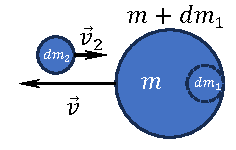
\includegraphics[width=0.9\linewidth]{image/Реактивное движение 2.pdf}
		\subcaption{ }
		\label{fig:3.1.1}
	\end{minipage}
	\hfill
	\begin{minipage}{0.49\linewidth}
		\centering
		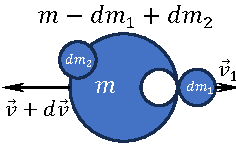
\includegraphics[width=0.9\linewidth]{image/Реактивное движение 1.pdf}
		\subcaption{ }
		\label{fig:3.1.2}
	\end{minipage}
	\caption{Реактивное движение}
	\label{fig:4}
\end{figure}

Запишем уравнение импульса (см. рис. \ref{fig:4}):
\[d\vec{p} = (m - dm_1 + dm_2)(\vec{v} + d\vec{v}) + dm_1\vec{v}_1 - (m\vec{v} + dm_2 \vec{v}_2)\]
\[d\vec{p} = \cancel{m\vec{v}} - \cancel{dm_1\vec{v}} + dm_2\vec{v} + md\vec{v} - \underbrace{(dm_1 - dm_2)}_{0}d\vec{v}  + \cancel{dm_1 \vec{v}} - \cancel{m\vec{v}} - dm_2 \vec{v}_2\]

Величины $dm_1$ и $dm_2$ бесконечно малые, поэтому при вычислении их разницы получим значение стремящиеся к нулю.
\[d\vec{p} = dm_2(\vec{v} - \vec{v}_2)\]

Изменение импульса системы:
\[ d\vec{p} = (m - dm_1 + dm_2)(\vec{v} + d\vec{v}) + dm_1\vec{v}_1 - dm_2\vec{v}_2 - m\vec{v} \]

Раскрываем скобки и упрощаем:
\[ d\vec{p} = \cancel{m\vec{v}} + md\vec{v} - dm_1\vec{v} \cancel{- dm_1d\vec{v}} + dm_2\vec{v} \cancel{+ dm_2d\vec{v}} + dm_1\vec{v}_1 - dm_2\vec{v}_2 - \cancel{m\vec{v}} \]

После отбрасывания малых второго порядка и сокращений:
\[ d\vec{p} = md\vec{v} - dm_1\vec{v} + dm_2\vec{v} + dm_1\vec{v}_1 - dm_2\vec{v}_2\]
\[\boxed{d\vec{p} = md\vec{v} + dm_1(\vec{v}_1 - \vec{v}) - dm_2(\vec{v}_2 - \vec{v})} \, \Big|:dt \]

Для удобства произведем замену переменных:
\begin{itemize}
	\item $u_1 = \vec{v}_1 - \vec{v}$ -- скорость отделяемого вещества, относительно тела;
	\item $u_2 = \vec{v}_2 - \vec{v}$ -- скорость присоединяемого вещества, относительно тела.
\end{itemize}
\[ \boxed{\frac{d\vec{p}}{dt} = m\frac{d\vec{v}}{dt} + \frac{dm_1}{dt}\vec{u}_1 - \frac{dm_2}{dt}\vec{u}_2} \]

\begin{center}
	\textbf{Уравнение Мещерского}
\end{center}
\[\boxed{m \dd{\vec{v}}{t} = \vec{F} - \vec{u}_1 \dd{m_1}{t} + \vec{u}_2 \dd{m_2}{t}},\]
\begin{center}
	где $\dd{m_1}{t}$ -- темп отсоединения вещества ($\dd{m_1}{t} < 0$), \\
	$\dd{m_2}{t}$ -- темп присоединения вещества ($\dd{m_2}{t} > 0$), \\
	$\vec{u}_1$ -- скорость отсоединяемого вещества относительно тела, \\
	$\vec{u}_2$ -- скорость присоединяемого вещества относительно тела, \\
	$\vec{F}$ -- сумма внешних сил, действующих на систему.
\end{center}

\textbf{Замечание:} Массу $m$ нельзя выносить за знак производной, так как она зависит от времени: $m = m(t) = m_0 + m_2(t) - |m_1(t)|$.

\textbf{Реактивная сила} - это реальная сила, действующая на тело со стороны отделяемого и присоединяемого вещества:
\[ \vec{F}_{\text{реакт}} = \vec{u}_1 \dd{m_1}{t} - \vec{u}_2 \dd{m_2}{t} \]

\subsubsection*{Примеры}
\begin{enumerate}
	\item \textbf{Прямоточный воздушно-реактивный двигатель (ПВРД)}

	В прямоточном воздушно-реактивном двигателе (ПВРД) воздух сжимается за счёт скоростного напора потока на входе, из чего следует, что ему нужна окружающая среда. В камере сгорания нагревается смесь сжатого воздуха и продуктов горения топлива. В выходном сопле газы расширяются, преобразуя тепловую энергию в кинетическую, что приводит к истечению газов с высокой скоростью.

	Для ПВРД уравнение реактивной силы принимает вид:
	\[\vec{F}_\text{р} = \vec{u}_1 \dd{m_1}{t} - \vec{u}_2 \dd{m_2}{t} = \dd{m_1}{t}(\vec{u}_1 - \vec{u}_2)\]
	где $\vec{u}_1$ -- скорость истечения газов, $\vec{u}_2$ -- скорость поступающего воздуха.

	\begin{figure}[H]
		\centering
		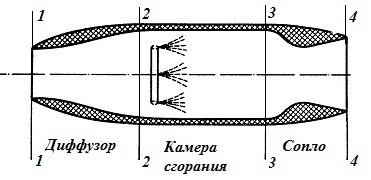
\includegraphics[width=0.7\linewidth]{image/ПВРД}
		\caption{Схема работы прямоточного воздушно-реактивного двигателя}
		\label{fig:3}
	\end{figure}

	\item \textbf{Твердотопливный реактивный двигатель (РДТТ)}

	В ракетном двигателе твердого топлива (РДТТ) топливо и окислитель содержатся в самом корпусе двигателя. При горении топлива образуются газы, истекающие через сопло:
	\[ \vec{F}_\text{р} = \vec{u} \dd{m}{t} \]
	где $\dd{m}{t} < 0$ (масса ракеты уменьшается).

	\item \textbf{Жидкостный ракетный двигатель (ЖРД)}

	В жидкостном ракетном двигателе отдельно хранятся топливо и окислитель, которые подаются в камеру сгорания. Преимущество -- возможность регулирования тяги:
	\[ \vec{F}_\text{р} = \vec{u} \dd{m}{t} + p_e A_e \]
	где $p_e$ -- давление на срезе сопла, $A_e$ -- площадь выходного сечения.
	\item \textbf{Турбореактивный двигатель (ТРД)}

	В турбореактивном двигателе воздух сжимается компрессором, затем в камере сгорания смешивается с топливом. Продукты сгорания расширяются в турбине и реактивном сопле:
	\[ \vec{F}_\text{р} = \vec{u}_\text{г} \dd{m_\text{г}}{t} - \vec{u}_\text{в} \dd{m_\text{в}}{t} \]
	где $\vec{u}_\text{г}$ -- скорость истечения газов, $\vec{u}_\text{в}$ -- скорость поступающего воздуха.

	\begin{figure}[H]
		\centering
		\includegraphics[width=0.8\linewidth]{image/РД}
		\caption{Схема турбореактивного двигателя}
		\label{fig:6}
	\end{figure}
\end{enumerate}
\newpage
\subsubsection*{Задача Циолковского}
Определить \textit{скорость}, которую развивает летательный аппарат под воздействием тяги ракетного двигателя, неизменной по направлению, при отсутствии всех других сил.

Введем начальные условия:
\[\begin{aligned}
	\vec{F} = 0 && \vec{v}(0) = 0 && m(0) = m_0 && \vec{u}_1 = \vec{u} = const && v(t) - ?
\end{aligned}\]
\[m \dd{\vec{v}}{t} = - \dd{m_1}{t} \vec{u}_1\]
\[\begin{aligned}
	\dd{m_1}{t} > 0 && \dd{m}{t} < 0 && \dd{m_1}{t} = - \dd{m}{t}
\end{aligned}\]

Спроецируем на ось полета ($x$):
\[x: \, m \dd{v}{t} = -\Big(\dd{m}{t}\Big)(-u) = - \dd{m}{t} u \, \Big| \cdot dt\]
\[m dv = -u dm\]
\[\int_{o}^{v} \, dv = - \int_{m_0}^{m} u \frac{dm}{m} \quad \Rightarrow\quad v = - u \ln\Big(\frac{m_0}{m}\Big)\]

Таким образом получаем \textbf{формулу Циолковского}:
\[\boxed{v = u \ln\Big(\frac{m_0}{m}\Big)}\]